\documentclass[a4paper,11pt]{report}
\usepackage{amsmath, amsthm, amssymb, amsfonts}
\usepackage{newlfont}
\usepackage{color}
%\usepackage[hypertex]{hyperref}
\usepackage{hyperref}
\usepackage[utf8x]{inputenc}
\usepackage{graphicx}
\usepackage{caption}
\usepackage{neuralnetwork}
\usepackage{tikz}
\usetikzlibrary{calc,fit,arrows}
\setlength{\evensidemargin}{0pt}
\setlength{\oddsidemargin}{0pt}
\setlength{\topmargin}{3pt}
\setlength{\textheight}{670pt}
\setlength{\textwidth}{450pt}
\setlength{\headsep}{5pt}
\setlength{\parindent}{0pt}
\setlength{\parskip}{1ex plus 0.5ex minus 0.2ex}

\newcommand{\norm}[1]{\left\Vert#1\right\Vert}
\newcommand{\abs}[1]{\left\vert#1\right\vert}
\newcommand{\ds}{\displaystyle}
\newcommand{\cost}{\mathrm{cost}}



\begin{document}

\title{Convolutional Neural Networks}
\author{Mihai Berbec}
\maketitle

\chapter{Convolutional Neural Networks}

\section{Convolutions}

\textbf{Convolution}

\begin{center}
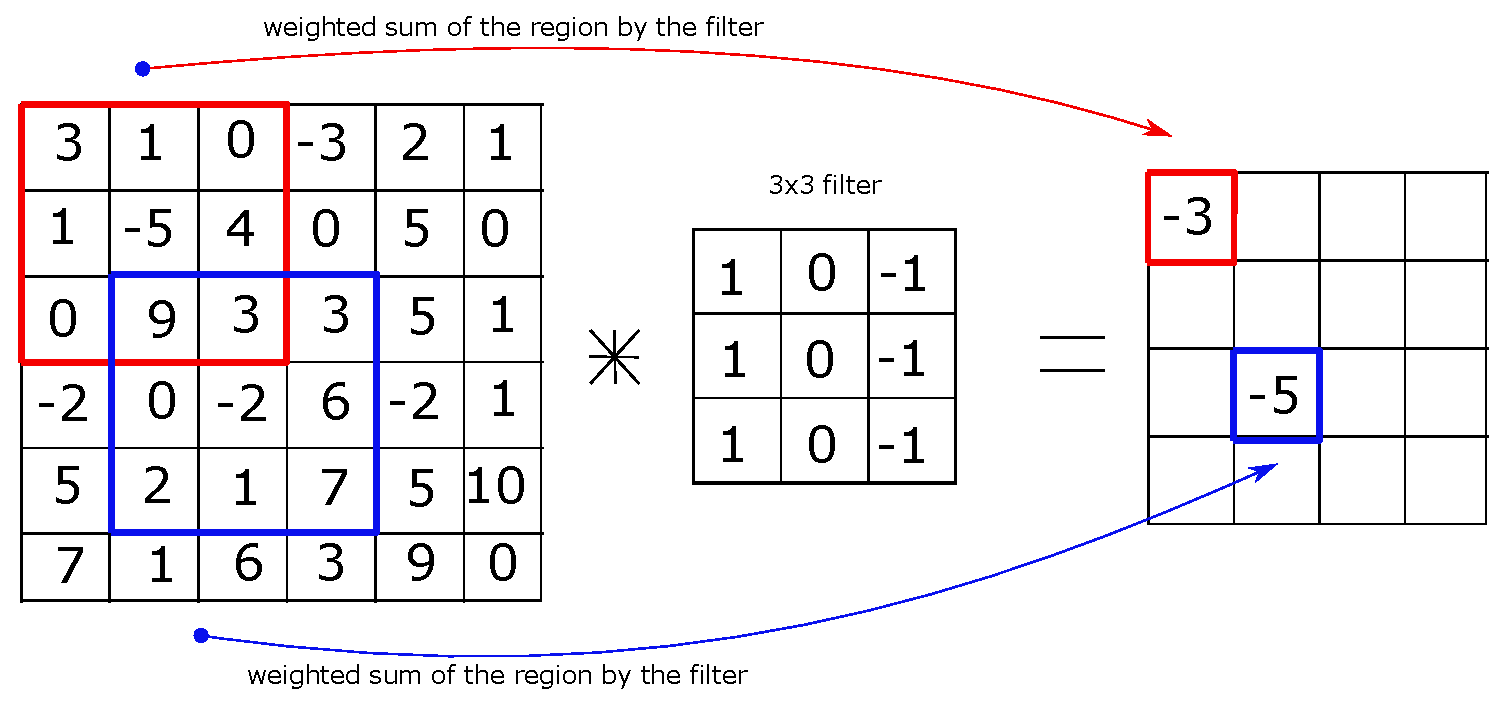
\includegraphics[height = 2in]{convolutions/convdef}
\end{center}

\textbf{Dimensions}: $(6, 6) * (3, 3) = (6-3+1, 6-3+1) = (4, 4)$, thus the image is shrinking with every convolution. Also, the information contained near the edges is not used.

If an $(n, n)$ image is convoluted with an $(f, f)$ filter, then the resulting image transforms \linebreak to $(n-f+1, n-f+1)$.

\textbf{Padding}: add a border of $p$ pixels around the edges (usually zeros). If the dimension of the original image is $(n, n)$, then the dimension of the padded image becomes $(n+2p, n+2p)$.

To preserve the input dimension we have to take $p = (f-1)/2$, where $(f, f)$ is the dimension of the filter ($f$ is usually odd).

\textbf{Stride}: how many pixels to move between two consecutive applications of the filter (in the figure above we have stride = 1).

In general, the result of a convolution $(n, n) * (f, f)$, with stride $s$ and padding $p$ is $$\left(\dfrac{n+2p-f}{s} + 1, \dfrac{n+2p-f}{s} + 1\right).$$

If the image has multiple channels, then the filter must have the same number of channels: $(n,n,3) * (f,f,3) = (n-f+1, n-f+1)$. Both the image region and the filter are cubes now, so the weighted sum is still possible.

Most of the time we apply many filters with the same size on an image and stack the resulting images as channels of new image:

$$\left.\begin{array}{ccc}
  (n,n,3) * (f,f,3) & = & (n-f+1, n-f+1)\\
  (n,n,3) * (f,f,3) & = & (n-f+1, n-f+1)
\end{array}\right\}\xrightarrow[]{\text{stack}} (n-f+1, n-f+1, 2).$$

\textbf{"Same" convolution}: dimension of the input equals dimension of the output.

\section{Convolutional layers}

Example of convolutional layer:

\begin{center}
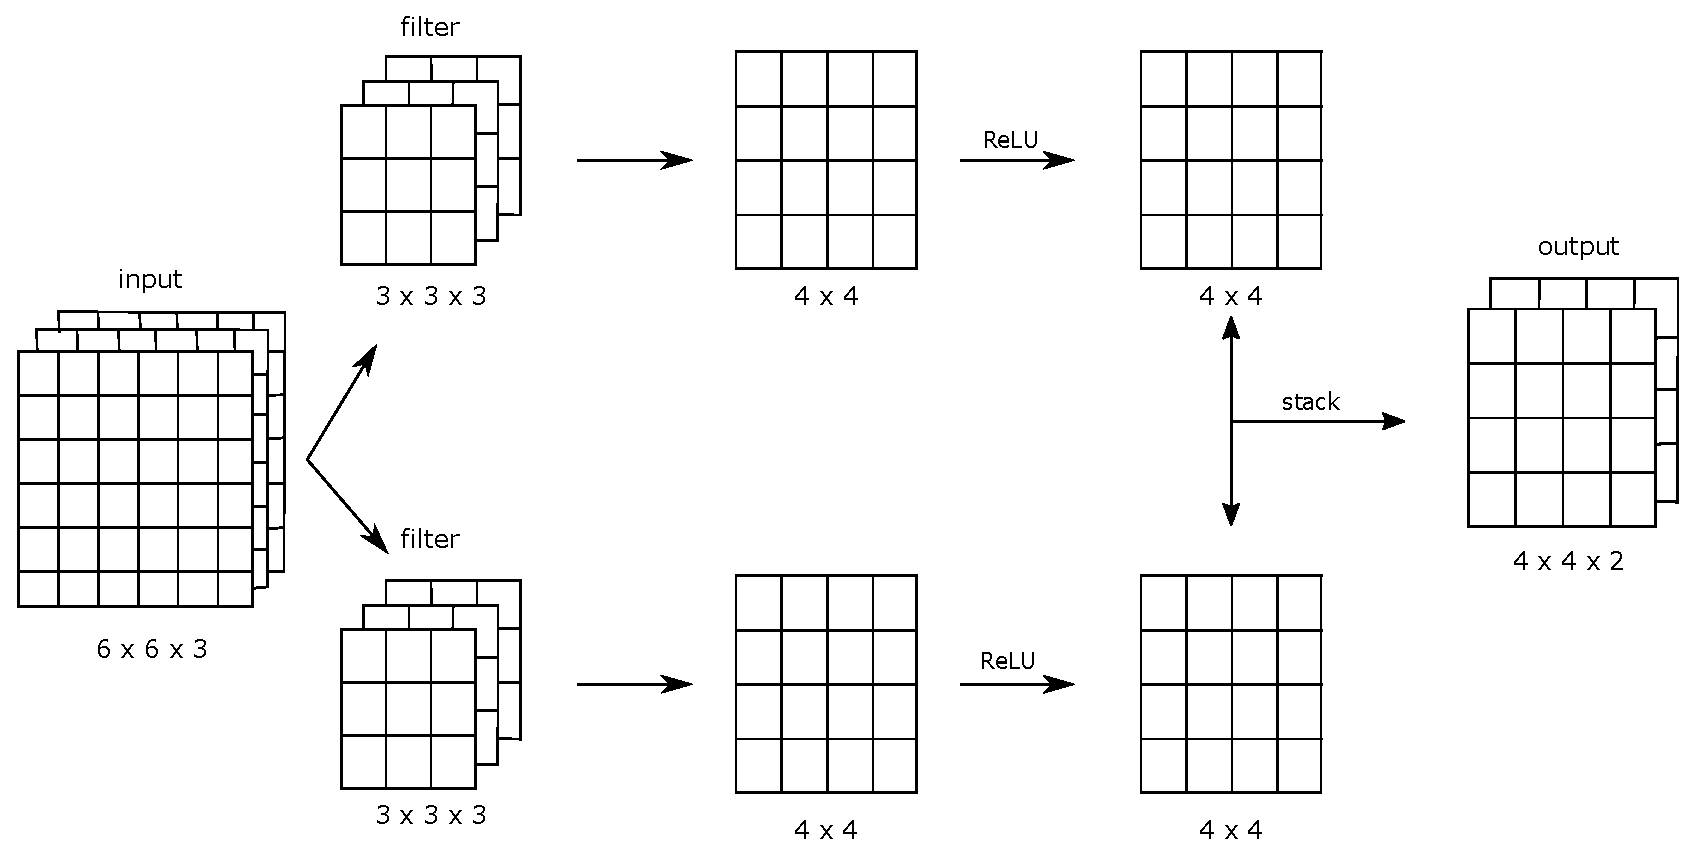
\includegraphics[height = 3in]{convolutions/convlayer}
\end{center}

The number of parameters of the layer is determined by the number and size of the filters, not by the size of the input image.

We fix the following notation:
\begin{itemize}
  \item $l$ = convolutional layer
  \item $f^l$  = filter size
  \item $p^l$ = padding size
  \item $s^l$ = stride
  \item $n_H^{l-1} \times n_W^{l-1} \times n_C^{l-1}$ = height $\times$ width $\times$ channels of the input coming from layer $l-1$
  \item $n_H^{l} \times n_W^{l} \times n_C^{l}$  = height $\times$ width $\times$ channels of the output
  \item $n_C^l$ = number of filters in the layer $l$
\end{itemize}
\break

Then: $$ n_{H/W}^l = \left\lfloor \dfrac{n_{H/W}^{l-1} + 2p^l - f^l}{s^l} +1 \right\rfloor,$$
and we have the following dimensions:
\begin{itemize}
  \item filters = $f^l \times f^l \times n_C^{l-1}$
  \item activations $a^l$ = $n_H^{l} \times n_W^{l} \times n_C^{l}$
  \item weights = $f^l \times f^l \times n_C^{l-1} \times n_C^{l}$
  \item biases = $1 \times 1 \times 1 \times n_C^{l}$
\end{itemize}

Example of convolutional neural network (CNN):

\begin{center}
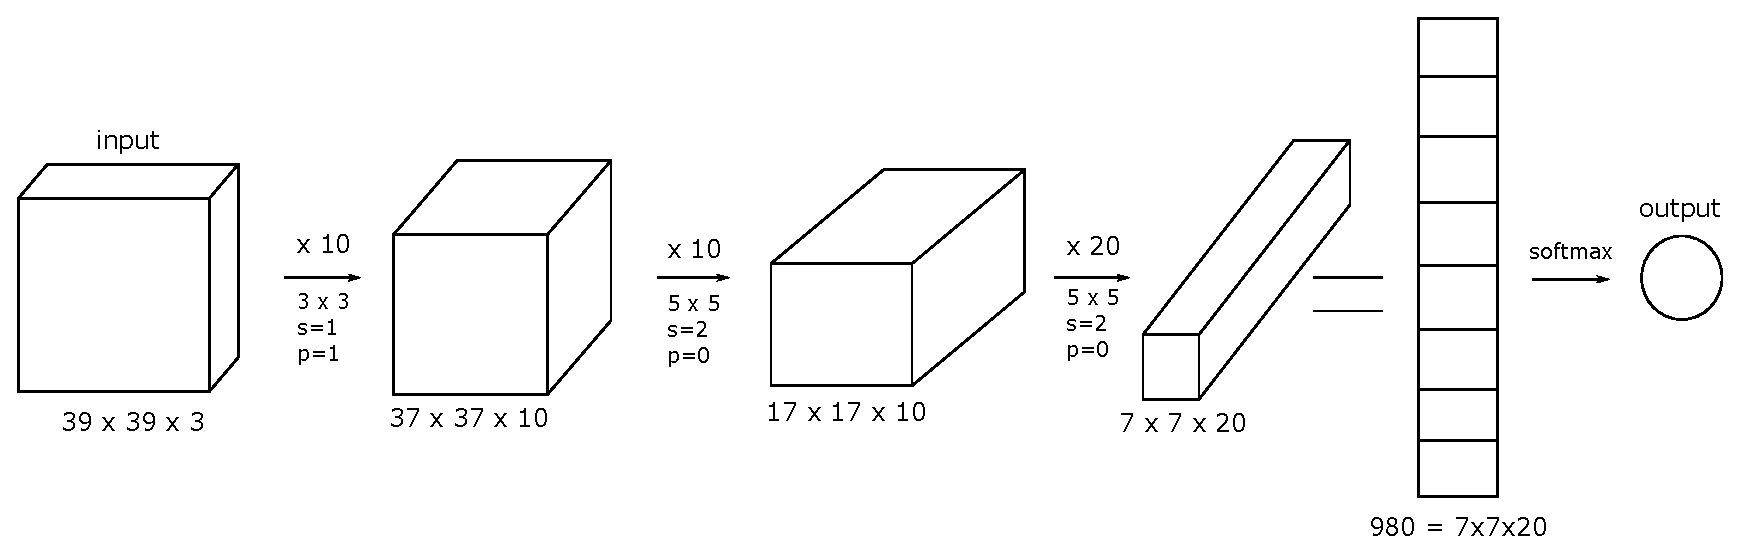
\includegraphics[width = 6in]{convolutions/convnet}
\end{center}

Why are convolutional networks good in practice ?
\begin{itemize}
  \item the number of learnable parameters is relatively small as many parameters are shared by the input nodes
  \item sparsity of connections: outputs depend only on a small number of inputs (less prone to overfitting, can train on smaller datasets)
\end{itemize}

\section{Pooling layers}

\hspace{0.5in}

\begin{center}
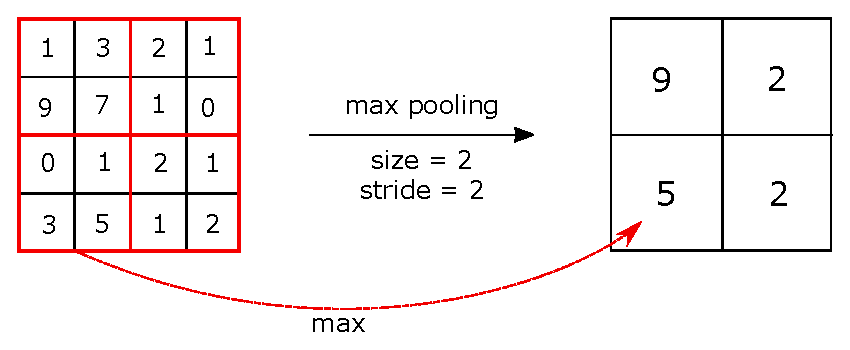
\includegraphics[width = 4in]{convolutions/maxpool}
\end{center}

Max pooling works very well in practice, but we can use min, average pooling, etc.

If the input image has multiple channels, pooling is done separately on each channel (thus it preserves the number of channels).

Pooling layers have no learnable parameters, they are used to reduce the image size.


\section{Classical convolutional networks}

\subsection*{LeNet-5}

Used to classify hand-written digits from the MNIST dataset (approx. 60k parameters).

\begin{center}
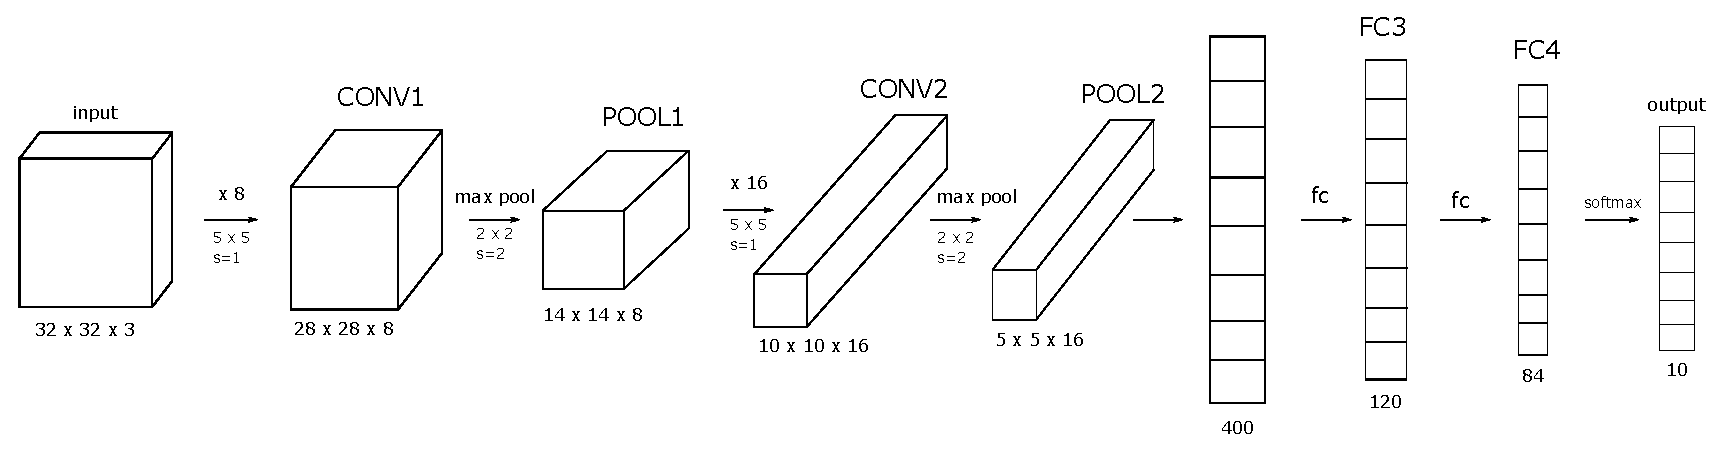
\includegraphics[width = 6in]{convolutions/lenet}
\end{center}

\begin{tabular}{|c|c|c|c|}
  \hline
  Layer & Shape & Size & Parameters\\
  \hline
  Input   & (32,32,3)  & 3072 & 0 \\
  Conv1   & (28,28,8)  & 6272 & 208 \\
  Pool1   & (14,14,8)  & 1586 & 0 \\
  Conv2   & (10,10,16) & 1600 & 416 \\
  Pool2   & (5, 5, 16) & 400  & 0 \\
  FC3     & (120,   1) & 120  & 48001 \\
  FC4     & (84,    1) & 84   & 10081 \\
  Softmax & (10,    1) & 10   & 841 \\
  \hline
\end{tabular}

\begin{itemize}
  \item pooling layers have no learnable parameters
  \item convolutional layers have few parameters comparing to the fully connected layers
  \item activations size goes down gradually trough the network
  \item image size decreases, but the number of channels increases
  \item in the original paper, sigmoid/tanh are used as activation functions (modern implementations use ReLU)
\end{itemize}


\subsection*{AlexNet}

Has approx. 60 millions parameters and uses ReLU as activation function. First successful convolutional network for images, trained on the ImageNet dataset.

\begin{center}
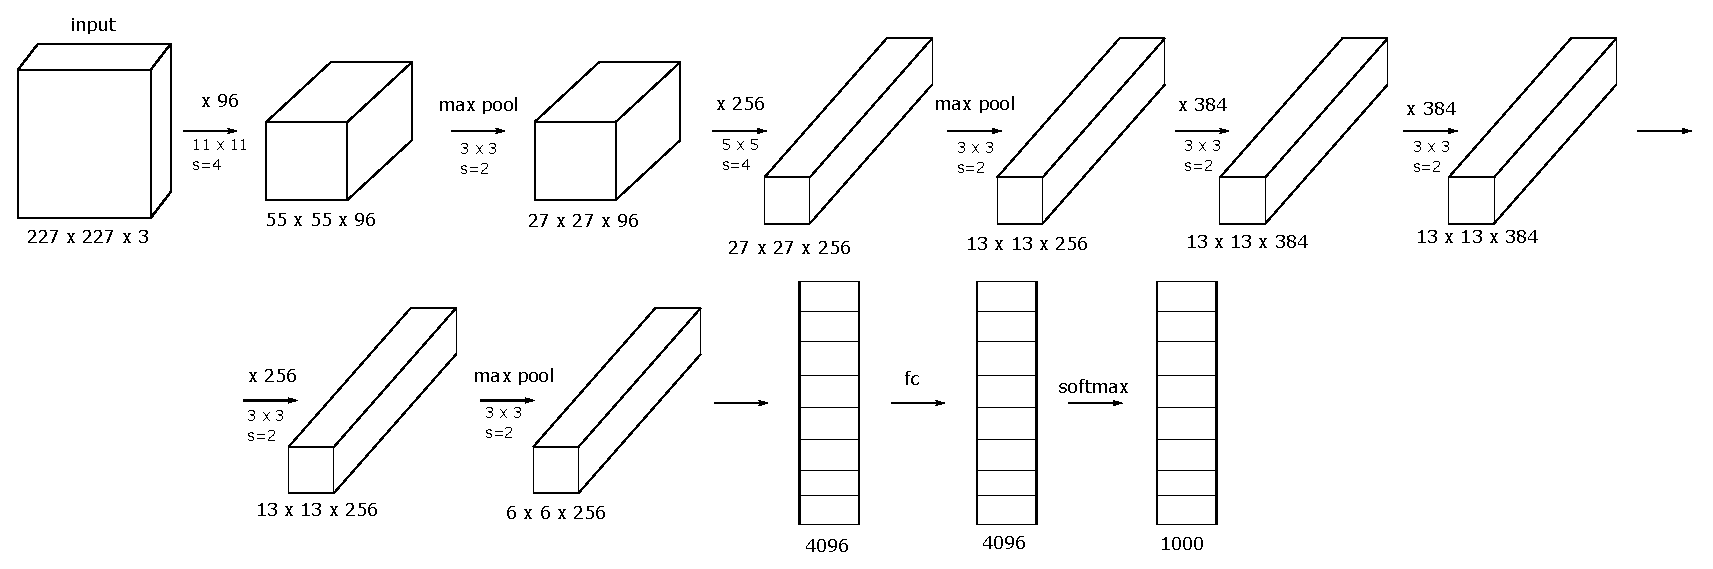
\includegraphics[width = 6in]{convolutions/alexnet}
\end{center}


\subsection*{VGG-16}

Has approx. 138 millions parameters. All convolutions are $3 \times 3$ with stride 1 and max pooling is $2\times 2$ with stride 2.

\begin{center}
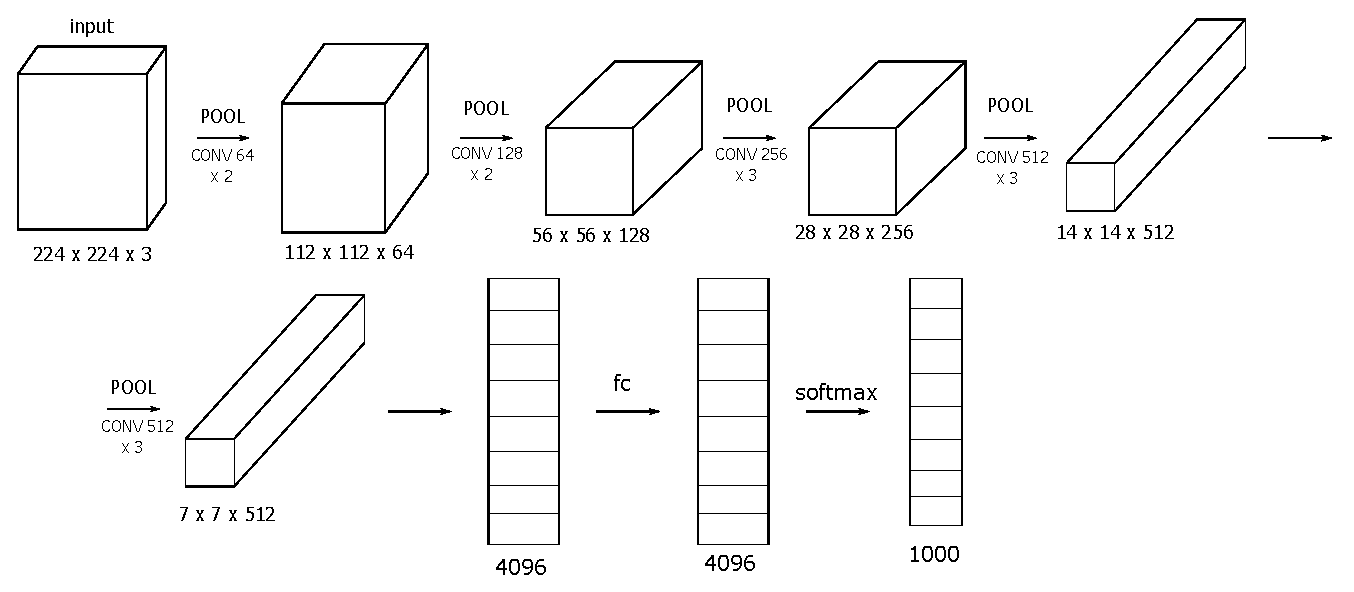
\includegraphics[width = 6in]{convolutions/vgg16}
\end{center}


\subsection*{ResNet - Residual Networks}

Very deep networks have an issue: vanishing/exploding gradients.

\hspace{0.3in}

Residual block

\begin{center}
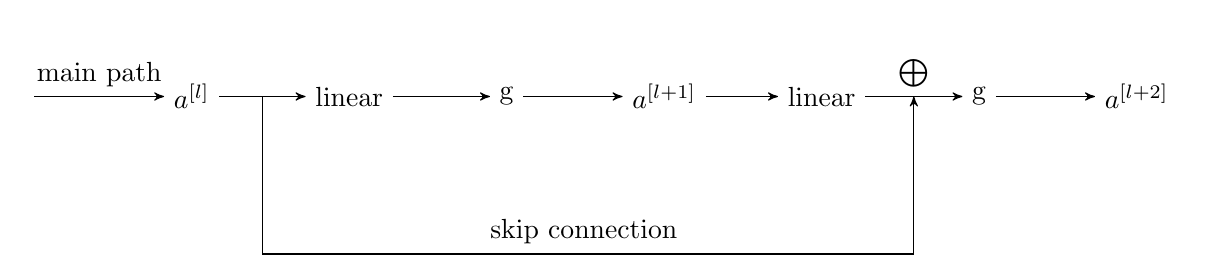
\begin{tikzpicture}[auto,node distance=2cm,>=stealth']

\node [coordinate]          (input)     {};
\node [right of = input]    (act_1)     {$a^{[l]}$};
\node [right of = act_1]    (linear_1)  {linear};
\node [right of = linear_1] (relu_1)    {g};
\node [right of = relu_1]   (act_2)     {$a^{[l+1]}$};
\node [right of = act_2]    (linear_2)  {linear};
\node [right of = linear_2] (relu_2)    {g};
\node [right of = relu_2]   (act_3)     {$a^{[l+2]}$};

\draw [->] (input) -- node (text) {main path} (act_1);
\draw [->] (act_1) -- node[name=start] {} (linear_1);
\draw [->] (linear_1) -- (relu_1);
\draw [->] (relu_1) -- (act_2);
\draw [->] (act_2) -- (linear_2);
\draw [->] (linear_2) -- (relu_2);
\path (linear_2) -- node (text) {$\bigoplus$} node[name=end] {} (relu_2);
\draw [->] (relu_2) -- (act_3);

%\draw [->] (linear_1) -- node[name=u] {}(relu_2);
\node [coordinate, below of=act_2] (measurements) {};
\draw [-] (start.south) |- node[pos=0.9] (text) {skip connection} (measurements);
\draw [->] (measurements) -| node {} node [near end] {} (end);
\end{tikzpicture}
\end{center}

On layer $l+2$, we have that: $$ a^{[l+2]} = g(z^{[l+2]} + a^{[l]}), $$ thus $z^{[l+2]}$ and $a^{[l]}$ must have the same dimension.

Residual networks are made of residual blocks. This particular architecture helps training very deep networks (e.g. ResNet: 34-layer residual network).

\subsection*{Inception networks}

\textbf{$1 \times 1$ convolutions} (networks in networks)
\begin{itemize}
  \item reduce the number of channels
  \item add non-linearity if keeping the same number of channels
\end{itemize}

\begin{center}
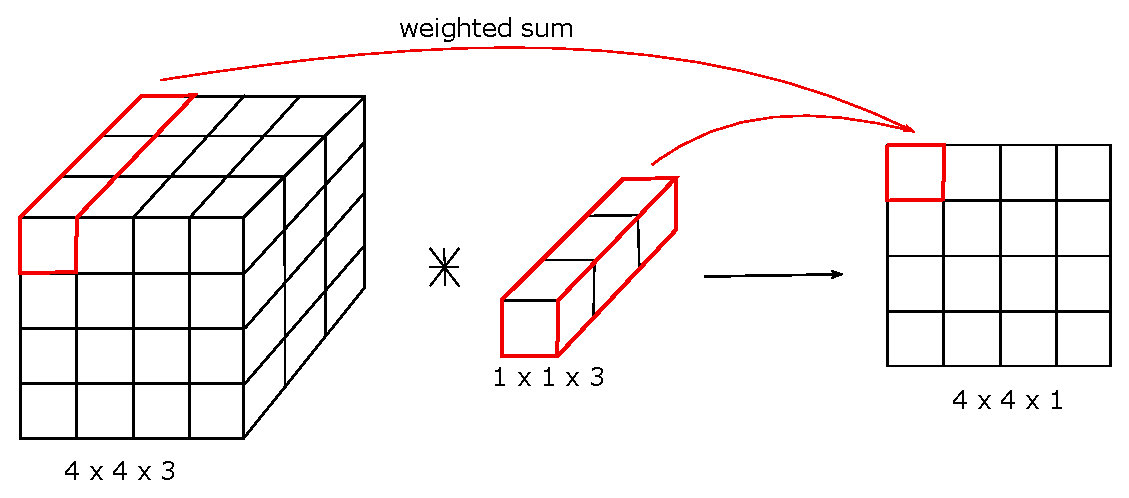
\includegraphics[width = 5in]{convolutions/1x1conv}
\end{center}

\textbf{Inception networks}

Assume we have to implement the following convolutional layer:

\begin{center}
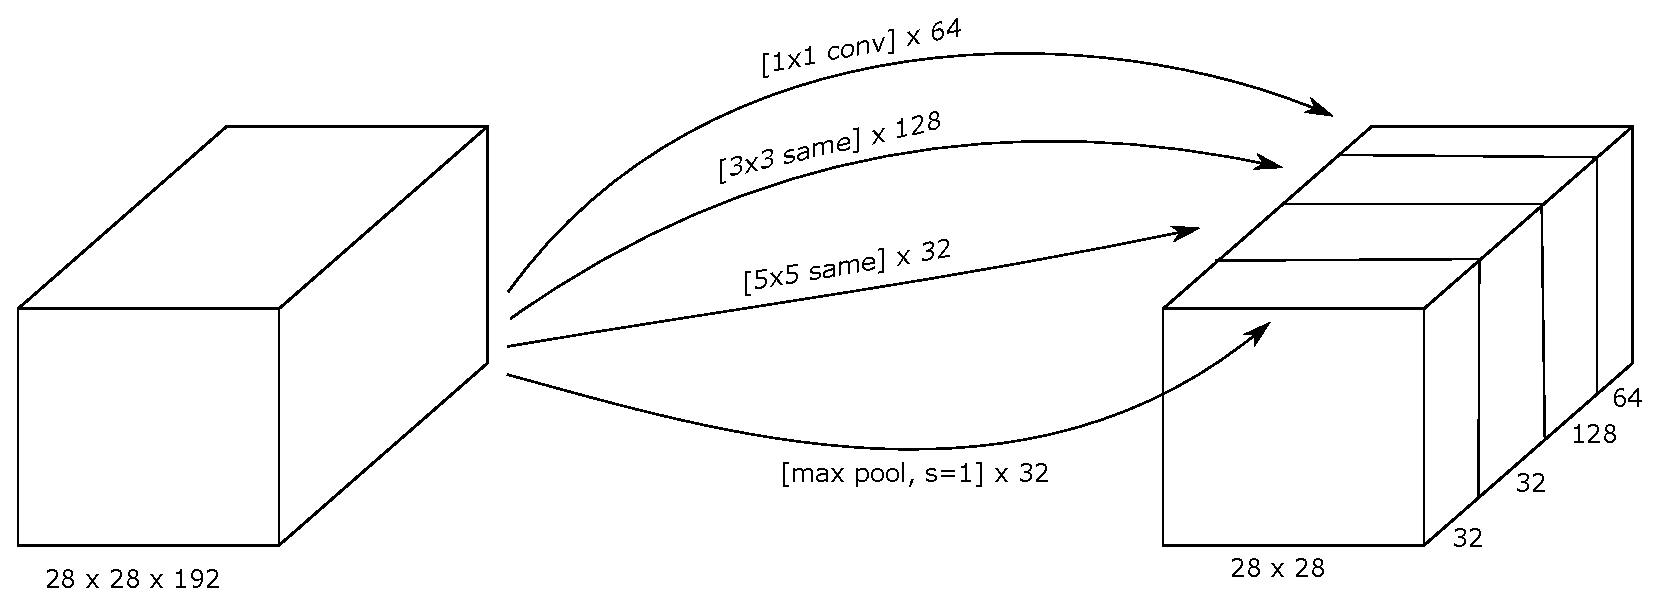
\includegraphics[width = 5in]{convolutions/inception1}
\end{center}

This layer is very expensive computationally: approx. 120 millions multiplications. Instead of $3\times 3$ and $5\times 5$ convolutions, we can use $1\times 1$ convolutions to reduce the number of channels and then run the corresponding convolutions.

\begin{center}
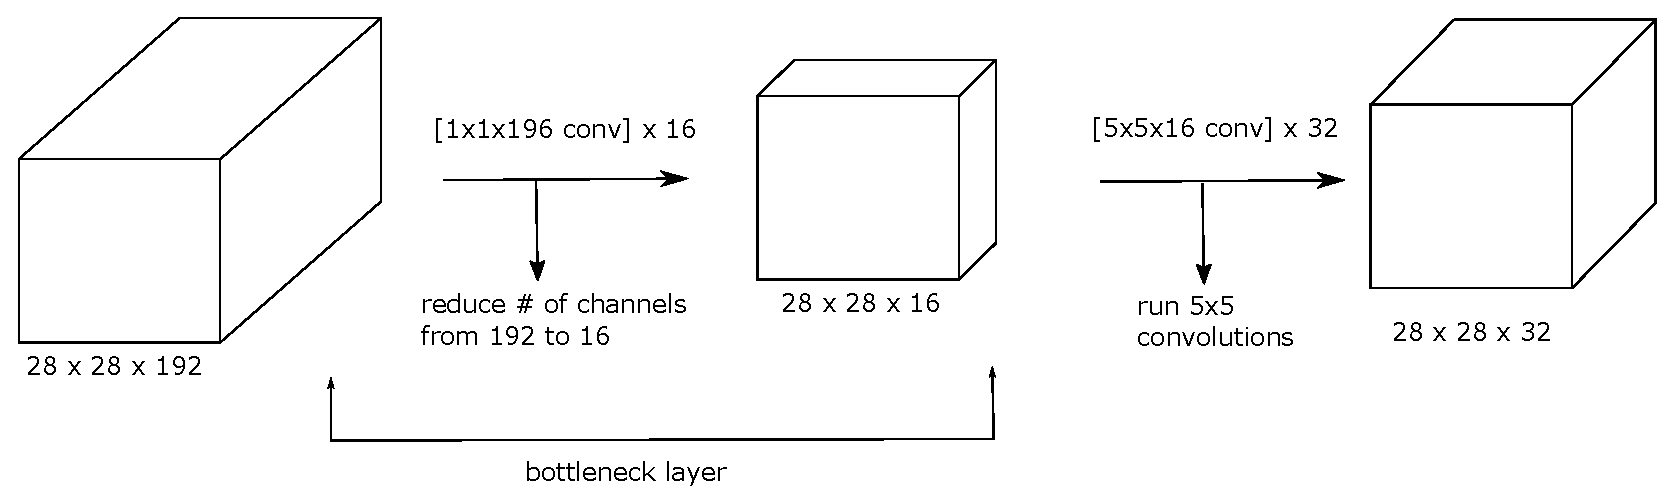
\includegraphics[width = 5in]{convolutions/bottleneck}
\end{center}

Compared to the layer above, this implementation has around 12.4 millions multiplications, almost 10 times less.

Using this kind of convolutions, we can implement an \textbf{inception module} as follows:

\begin{center}
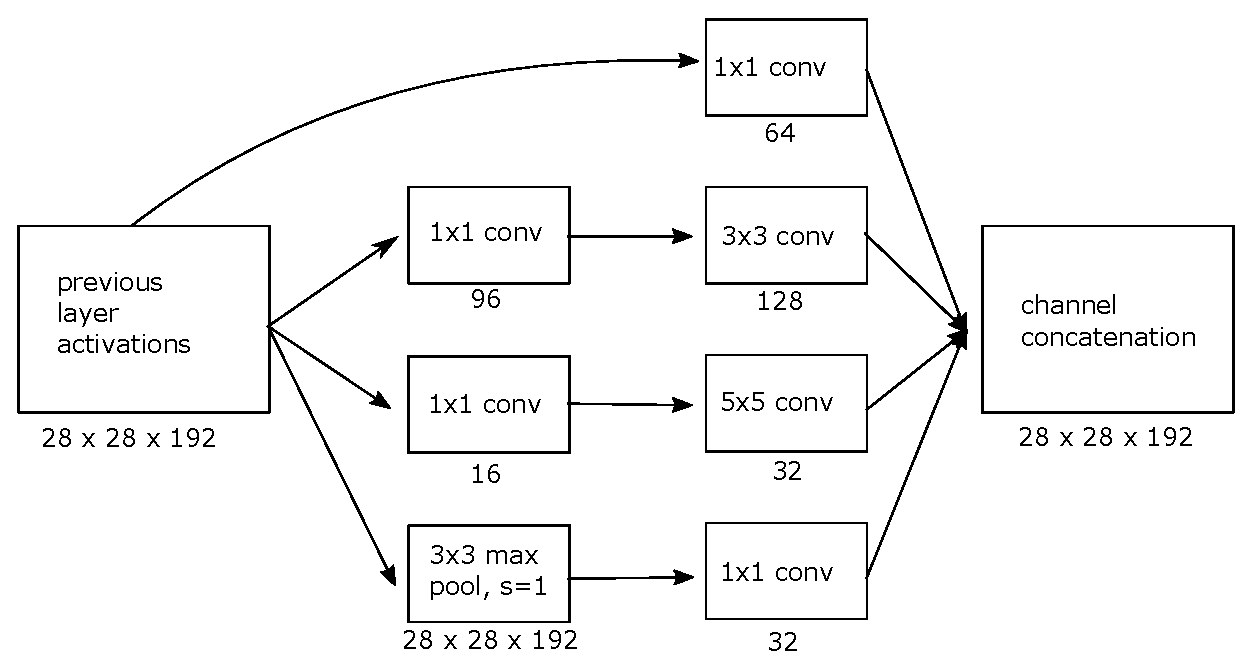
\includegraphics[width = 5in]{convolutions/inception_module}
\end{center}

Inception network (\textbf{googLeNet}) - put together many inception modules (9 modules up to pooling), plus some additional side branches with softmax output to ensure that intermediate features are not too bad for prediction (this has a regularizing effect and prevents overfitting).


\subsection*{Data augmentation}

\begin{itemize}
  \item horizontal flip
  \item random cropping
  \item rotation, shearing, wrapping (not too often)
  \item color shifting (RGB)
\end{itemize}


\section{Object Detection}

Localization - classify the image and localize the main object (as a bounding box). We can use a simple classifier with a softmax layer with size equal to the number of classes.

\begin{center}
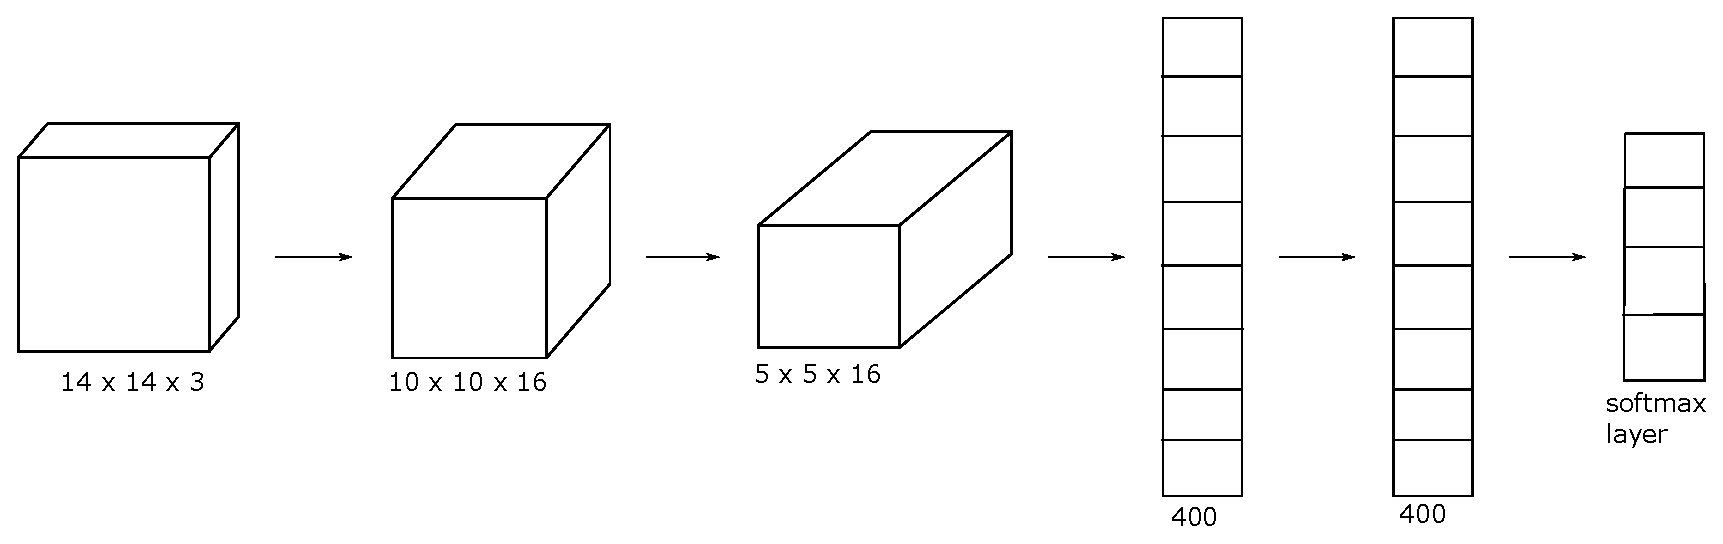
\includegraphics[width = 5in]{convolutions/classifier}
\end{center}

Detection - find all objects in the image and draw bounding boxes around them (many objects, different categories).

Sliding window detection:
\begin{itemize}
  \item slide different size windows though an image and use a classifier to find objects (this method has a huge computational cost)
  \item can be implemented using convolutions
\end{itemize}

To do this, we turn the fully connected layers of the previous classifiers into convolutional layers.

\begin{center}
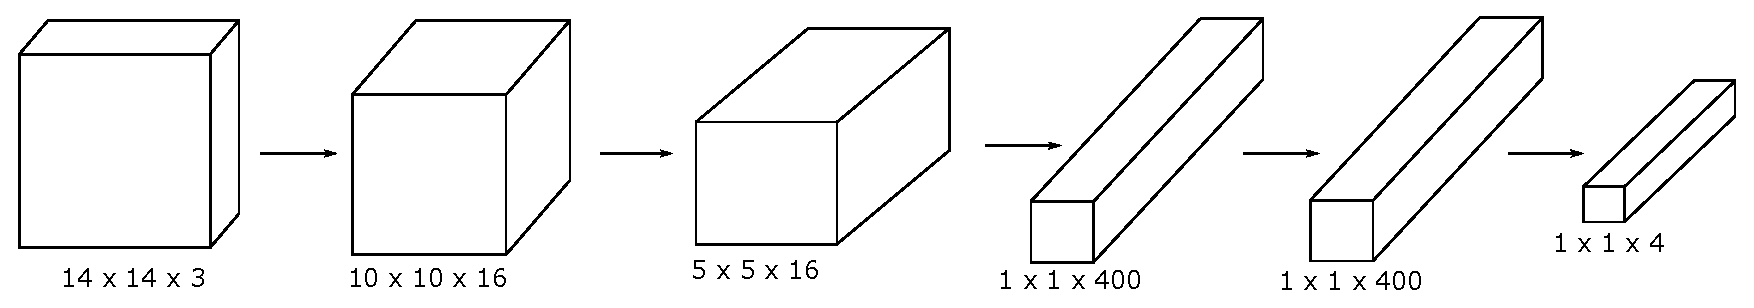
\includegraphics[width = 5in]{convolutions/slide_class}
\end{center}

For larger images, we apply the same network on each sliding window and put together the outputs.

\begin{center}
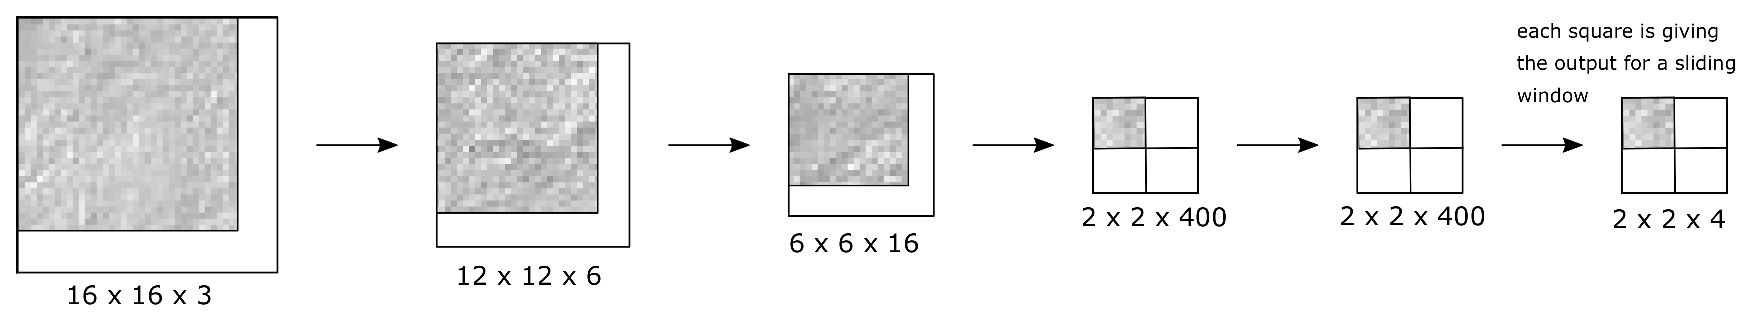
\includegraphics[width = 5in]{convolutions/slides}
\end{center}

This still has an issue: the position of bounding boxes is not very accurate.

\subsection*{YOLO object detection algorithm}

YOLO (You Only Look Once) predicts the bounding boxes of objects in the image.

Assume we start with an $100\times 100$ image and we have 3 different object classes we want to detect. We add a finer grid on the image and apply an image localization network (as the previous classifier) on each grid cell.

\begin{center}
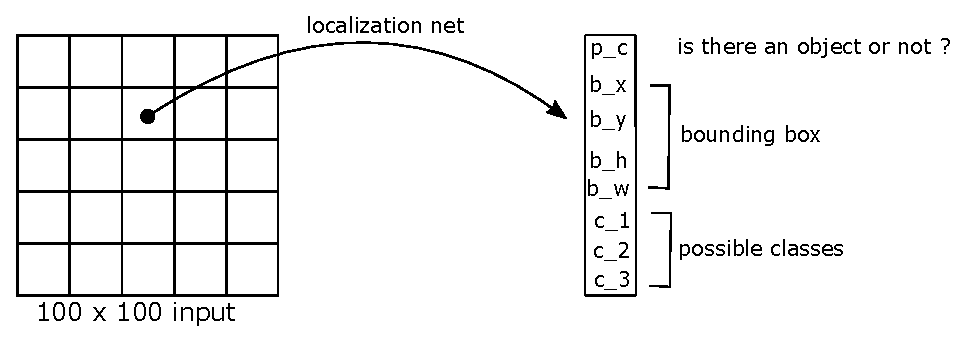
\includegraphics[width = 4in]{convolutions/yolo_grid}
\end{center}

Thus for each cell of the input image we get an 8-dimensional vector $y = [p_c, b_x, b_y, b_h, b_w, c_1, c_2, c_3]$, where:
\begin{itemize}
  \item $p_c$ is 0 or 1, saying if there is an object or not in the cell,
  \item $ b_x, b_y, b_h, b_w$ is the bounding box of the object,
  \item $c_1, c_2, c_3$ is a vector indicating the class of the object (an entry is 1 and the rest are 0).
\end{itemize}

We use these 8-dimensional vectors as labels for training a convolutional network. If an object is spread over multiple cells, we assign the object to the cell that contains its center.

As in the previous figure, if we put a $5\times 5$ grid on the input images, we get 25 output vectors arranged in a $5\times 5 \times 8$ matrix:

\begin{center}
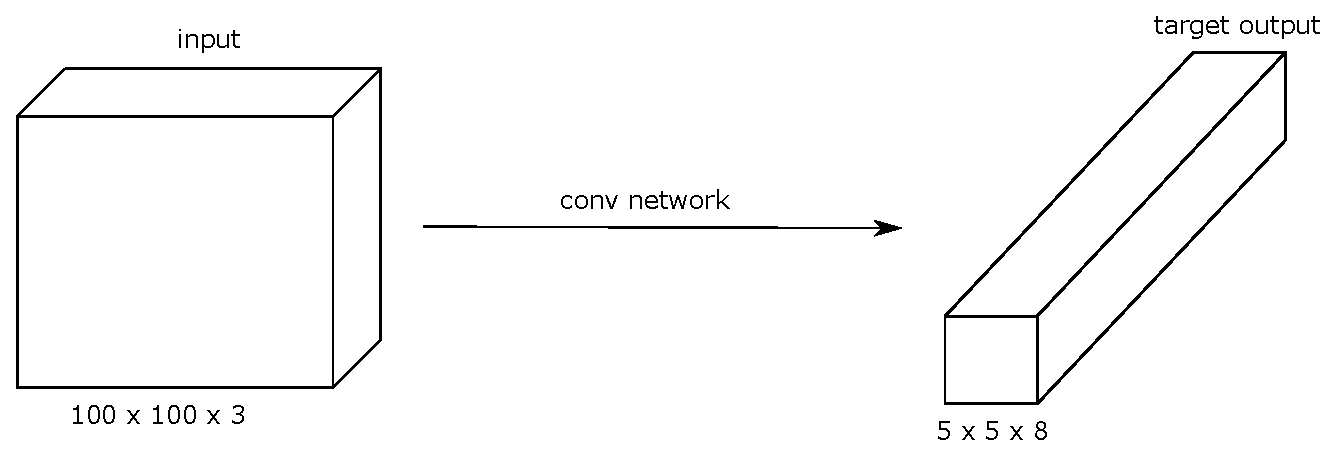
\includegraphics[width = 4in]{convolutions/yolo_target}
\end{center}

We use IOU (intersection over union) to measure detection accuracy.
\begin{itemize}
  \item IOU measures the overlap of two bounding boxes,
  \item in our case, IOU equals the ratio between the area of the intersection and the area of the union of the ground truth and predicted bounding boxes,
  \item usually, if IOU $\ge 0.5$, the prediction is assumed to be correct.
\end{itemize}

So far, this approach works better than the sliding window, but there are still issues: we can find multiple detections of the same object if the grid is fine.

\subsubsection*{Non max suppression}

Assume we have a star-like object to detect in the input image:

\begin{center}
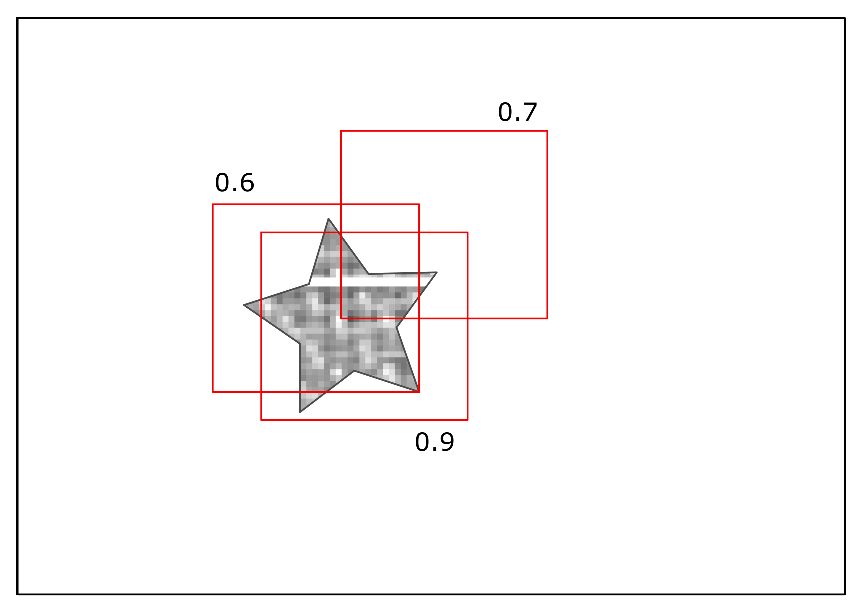
\includegraphics[width = 2.5in]{convolutions/yolo_nonmax}
\end{center}

As we see in the image, we have 3 bounding boxes containing the object ($p_c = 1$ and the same class). To get the correct bounding box we use the non max suppression principle.
\begin{itemize}
  \item take the most confident prediction (e.g. that one with IOU $= 0.9$) and mark it,
  \item look at the remaining bounding boxes and suppress those with high IOU,
  \item the final predictions will be the marked ones.
\end{itemize}

There is another issue here: each of the grid cells can detect only one object.

\subsubsection*{Anchor boxes}

Pre-define different shapes called anchor boxes and allow the algorithm to specialize in detecting objects similar to these anchor boxes.

More specifically, for each grid cell we define a target output vector $y = [y_1, y_2, \ldots, y_n]$, where $y_i$ are similar to the output defined above, that can encode many objects in the same grid cell.

\begin{center}
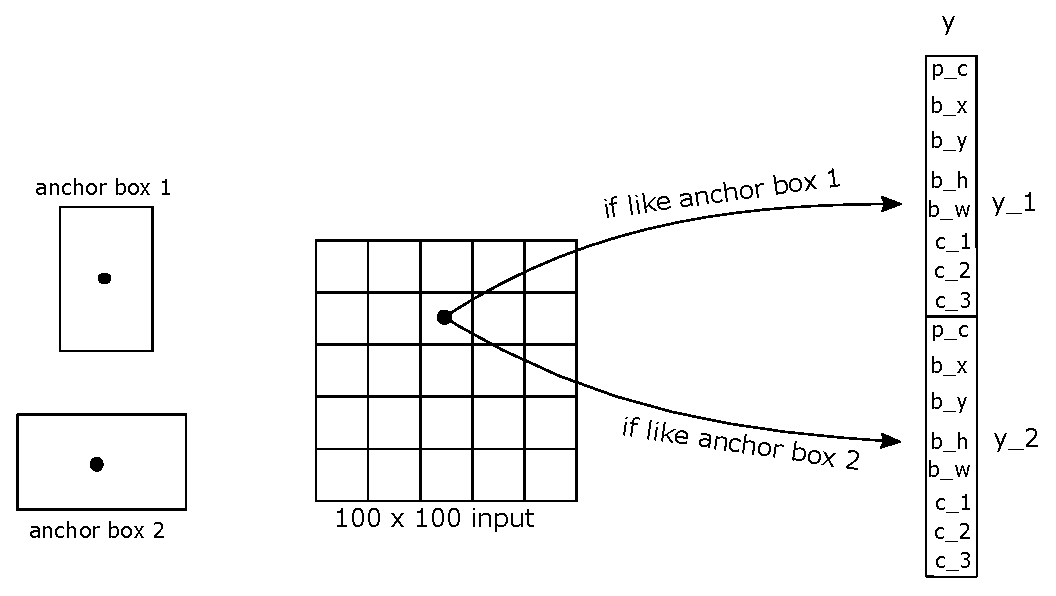
\includegraphics[width = 4in]{convolutions/yolo_anchor}
\end{center}

Now, each object in the training image is assigned to the cell that contains object's midpoint and anchor box with the highest IOU.

\subsubsection*{The YOLO algorithm}

For simplicity, assume that we have 3 classes and 2 anchor boxes as before.

\begin{itemize}
  \item start with an input image $x$ and add a fine grid on it (e.g. $5\times 5$ grid), 
  \item for each grid cell, run an image localization algorithm to get the target output $y$ (in our case, the size of $y$ is $5\times 5 \times 2 \times 8$ or $5\times 5 \times 16$),
  \item train a convolutional network with input $x$ and output $y$:
    \begin{center}
    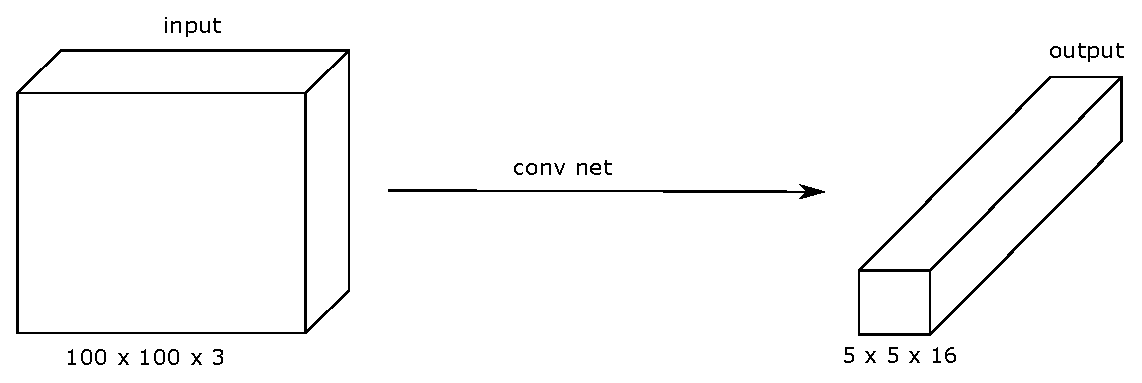
\includegraphics[width = 2.5in]{convolutions/yolo_target_alg}
    \end{center}
  \item run non-max suppression on all bounding boxes predicted for the input image and get the correct predictions.    
\end{itemize}


\subsection*{Region Proposal (R-CNN)}

R-CNN: if running a trained classifier across sliding windows, there are many windows containing no objects, so no need for detection. Instead, we can pick some regions where it makes sense to run the detector. To do this, we can use a segmentation algorithm based on pixel clustering (this can be very slow, as it may propose many regions and one region is classified at a time).

Fast R-CNN: use convolutional implementation of sliding window to classify all proposed regions at once. It is faster than R-CNN algorithm. 

Faster R-CNN: use convolutional networks to propose the regions instead of the clustering segmentation algorithm (faster than R-CNN, but somehow slower than YOLO).


\section{Face Recognition}

One shot learning: there exists only one image for every person. We need to learn a similarity function which tells if two images are of the same person or not. 

\subsection*{Siamese networks}

Use two identical convolutional networks to extract feature encodings of the input images and put them together using a similarity function (which can be seen as a cost function).

\begin{center}
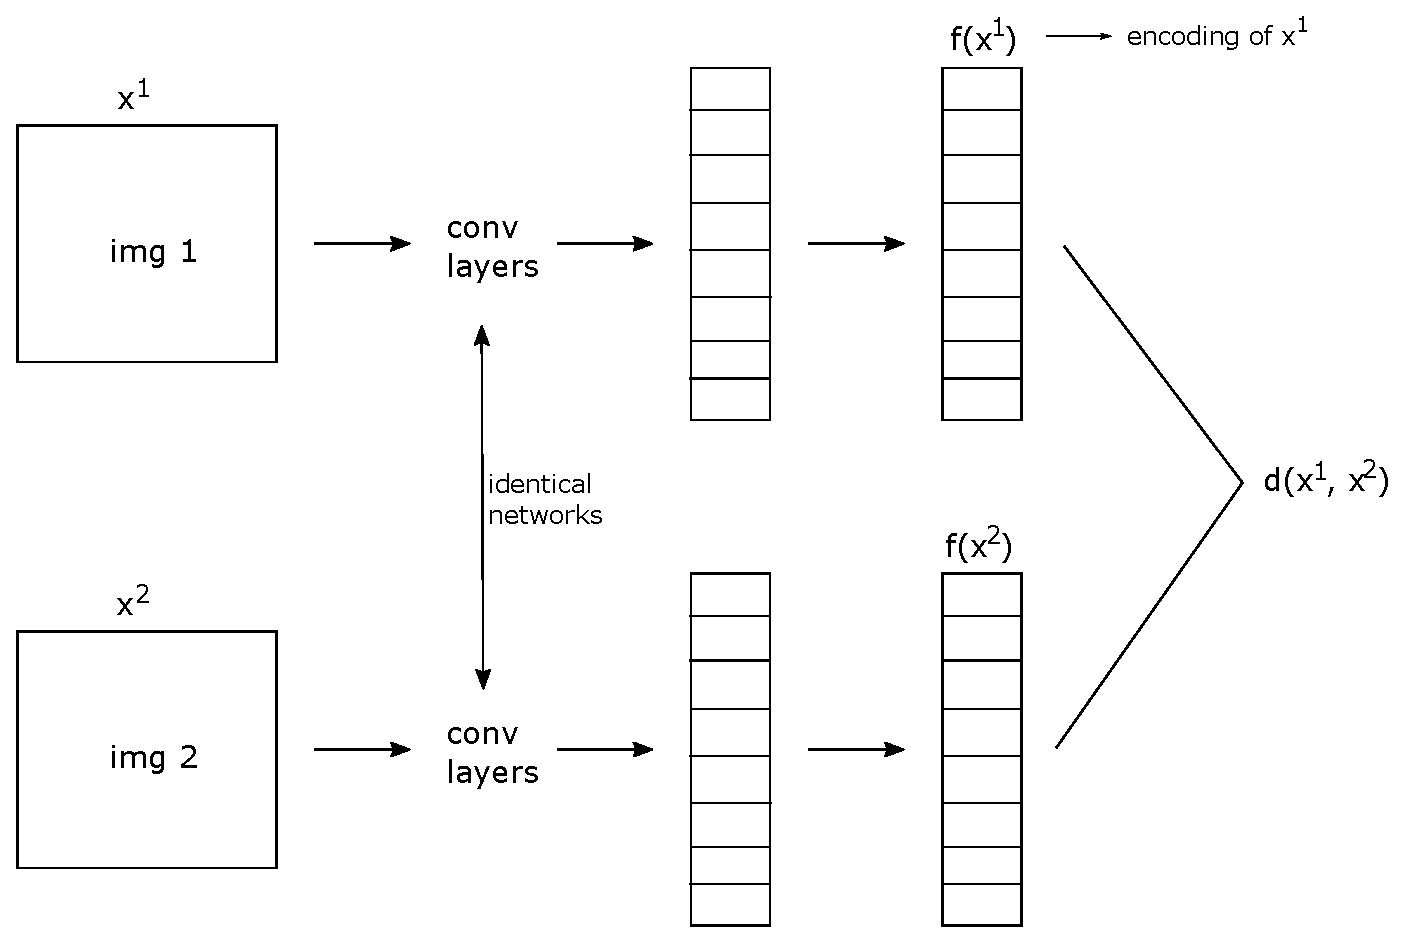
\includegraphics[width = 4in]{convolutions/siamese}
\end{center}

The similarity distance $d$ between the input images $x^1$ and $x^2$ is defined as the distance between the feature encodings $f(x^1)$ and $f(x^2)$: $$ d(x^1, x^2) = \norm{f(x^1) - f(x^2)}_2^2.$$

Learn network's parameters in such a way that:
\begin{itemize}
  \item if $x^i$ and $x^j$ are the same person, then $\norm{f(x^i) - f(x^j)}_2^2$ is small,
  \item if $x^i$ and $x^j$ are the different person, then $\norm{f(x^i) - f(x^j)}_2^2$ is large.
\end{itemize}

\subsubsection*{Triplet loss}

The triplet loss function requires a three images as input: anchor ($A$), positive ($P$), negative ($N$), where the anchor and the positive are similar and the anchor and the negative are different. The
objective is to find parameters such that: 
$$ \norm{f(A) - f(P)}_2^2 + \alpha \le \norm{f(A) - f(N)}_2^2,$$
where $\alpha$ is a positive number called margin. 

For a triplet $(A, P, N)$, the triplet loss function is defined as: 
$$ \mathcal{L}(A, P, N) = \max\left\{ \norm{f(A) - f(P)}_2^2 - \norm{f(A) - f(N)}_2^2 + \alpha, 0 \right\}.$$

If the triplets $(A, P, N)$ are randomly chosen, then $d(A, P) + \alpha \le d(A, N)$ is easily satisfied. Instead, choose triplets that are "hard" to train on, i.e. $d(A, P) \sim d(A, N)$ (see FaceNet, 2015).  






















\end{document} 